% Chapter02

\section{PWM逆变器工作原理}
\setcounter{figure}{0}
\setcounter{table}{0}
\subsection{二级标题}

\subsection{三级标题}
正文中的公式。采用公式编辑器进行编辑。

\begin{equation}
E_{i}=\int \left | c_{i}(t) \right | ^2dt=\sum_{j=1}^{m}\left | c_{ij}\right | ^2  
\end{equation}

其中,$c_{ij}(i=1,2,\dots,n,j=1,2,\dots,m)$表示IMF的离散点的幅值,
$m$为信号采样点的数目。(公式中涉及的字母所代表的物理量要全部指明。右对齐,符号大小在公式编辑器中
尺寸栏中的“define”下的‘full’项选12,其他默认)

正文中的图{\zihao{5}(图题在图的下方,居中,图题文字为五号宋体,图中文字为小五号)}

\begin{figure}[htbp]
	\centering
	\begin{minipage}{0.49\linewidth}
		\centering
		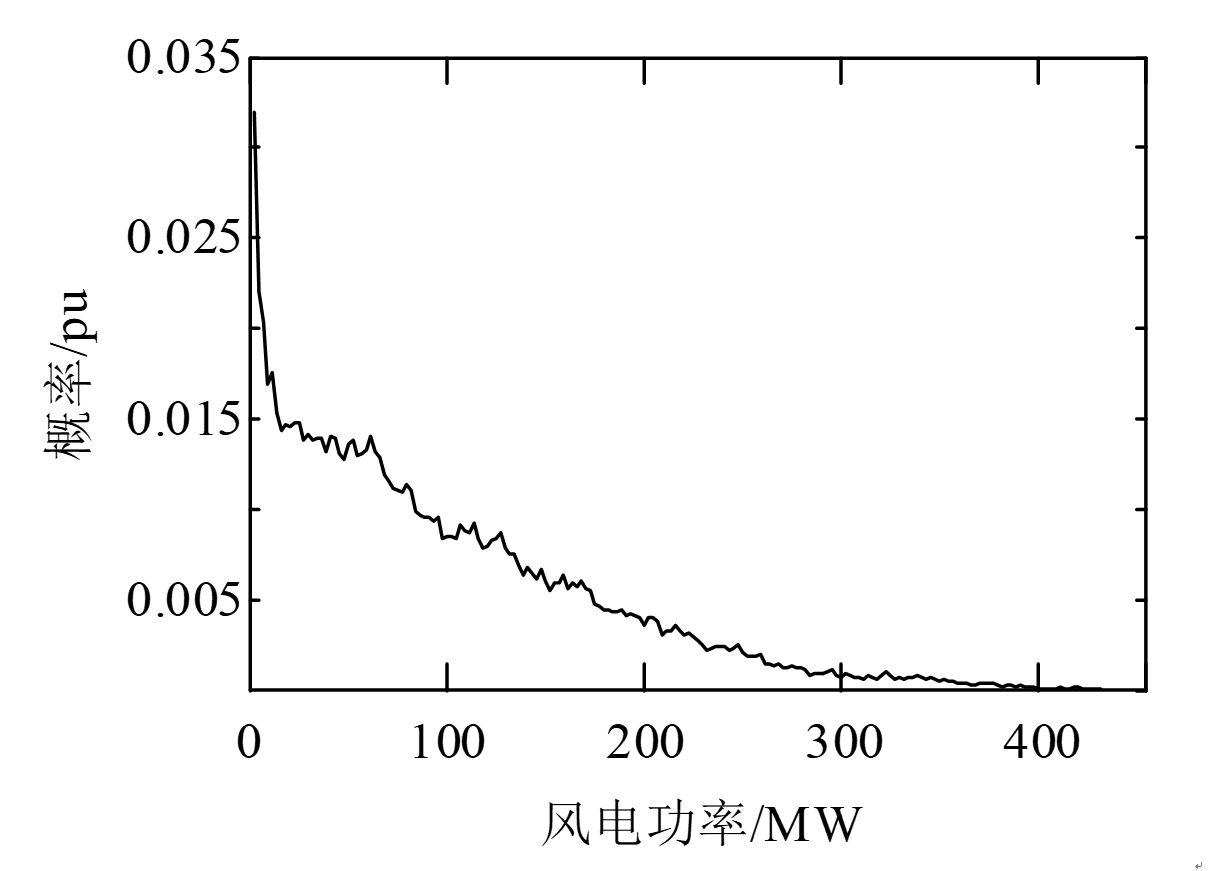
\includegraphics[width=0.9\linewidth]{figures/功率波动概率密度分布曲线}
		\caption{\zihao{5}功率密度概率密度分布曲线}
		\label{功率密度概率密度分布曲线}%文中引用该图片代号
	\end{minipage}
	%\qquad
	\begin{minipage}{0.49\linewidth}
		\centering
		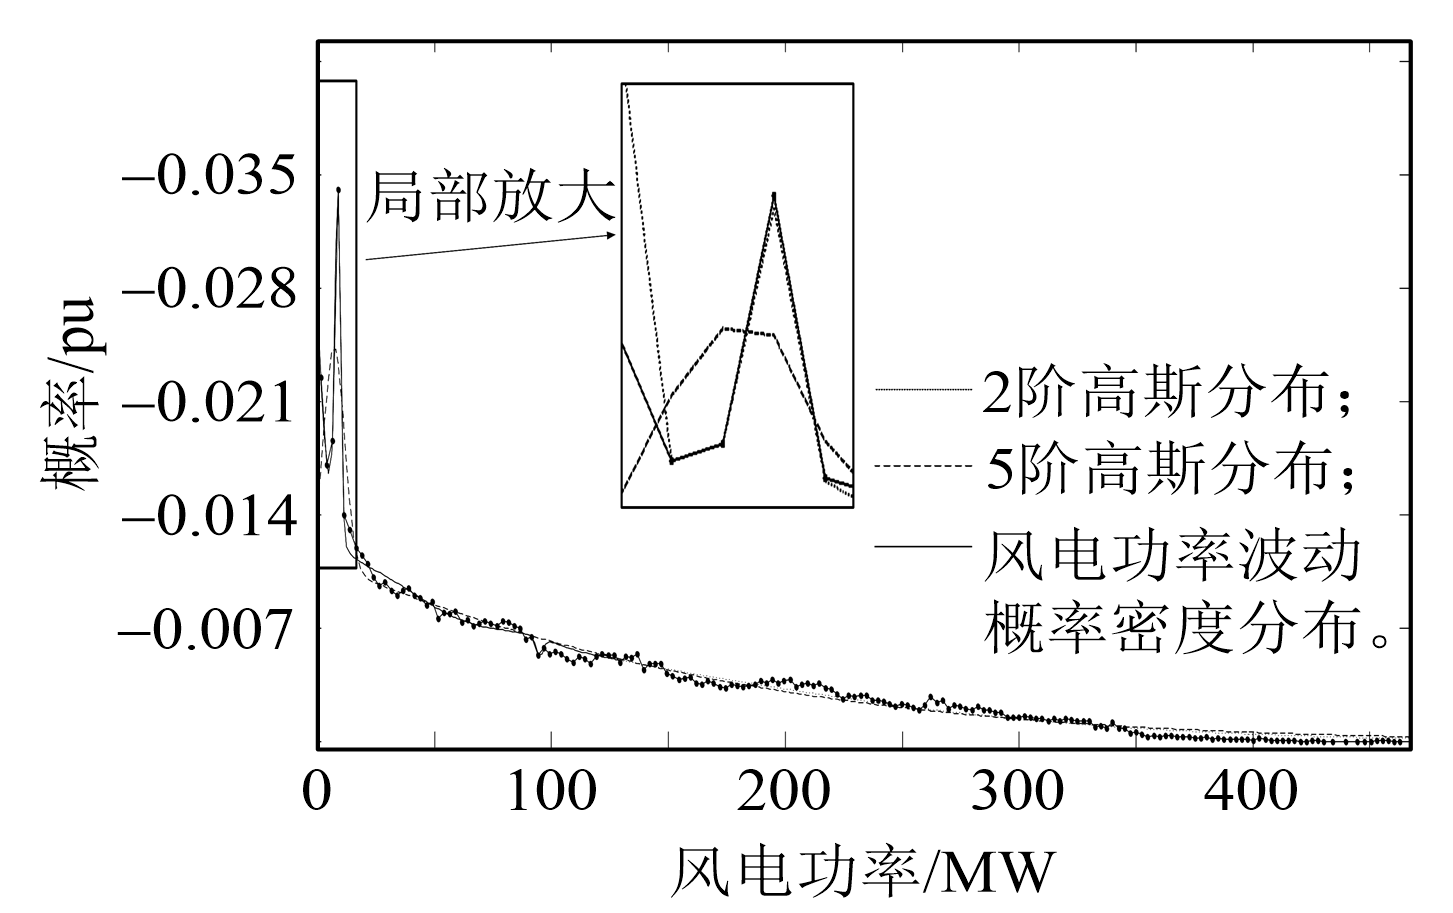
\includegraphics[width=\linewidth]{figures/功率波动概率密度分布拟合曲线}
		\caption{\zihao{5}功率密度概率密度分布拟合曲线}
		\label{功率密度概率密度分布拟合曲线}%文中引用该图片代号
	\end{minipage}
\end{figure}

\begin{figure*}
  \centering
    \subcaptionbox{subcaption1}{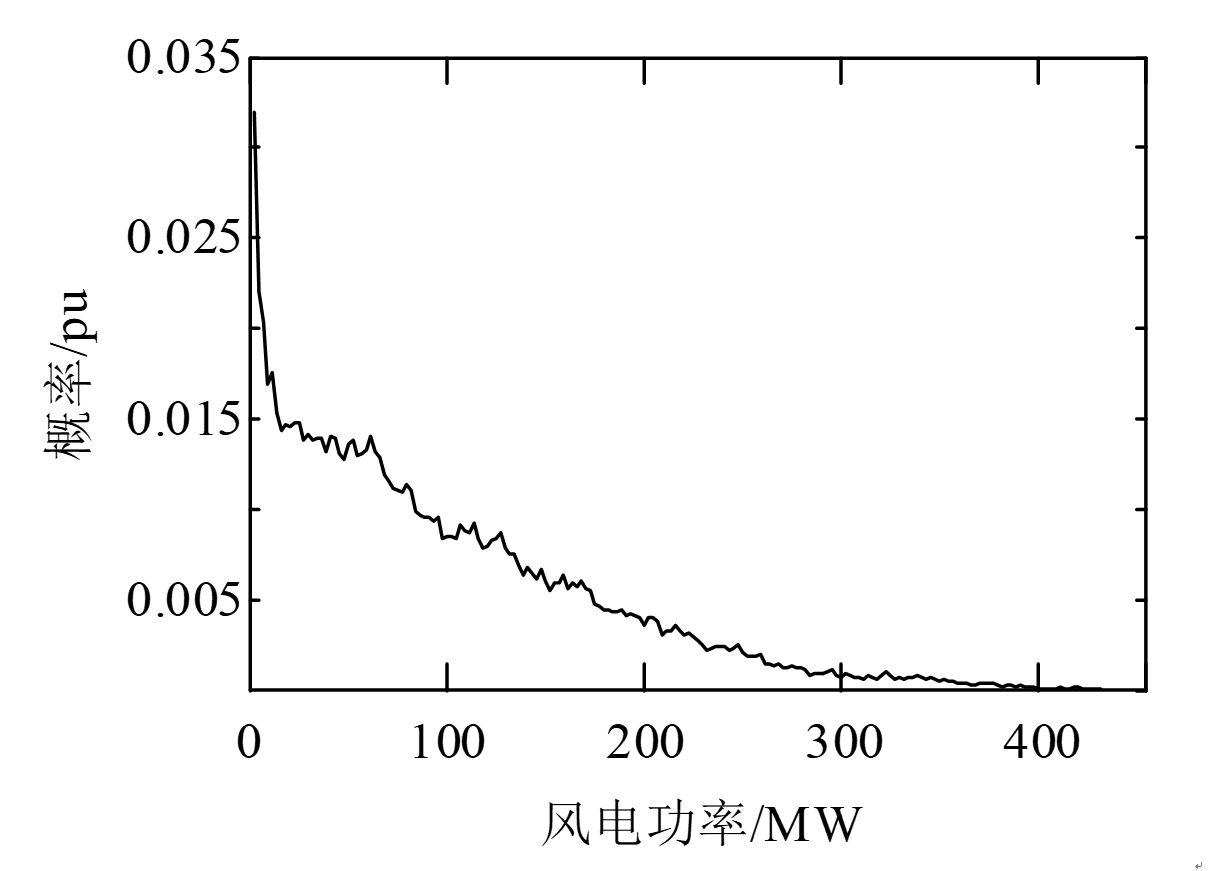
\includegraphics[width = 0.3\textwidth]{figures/功率波动概率密度分布曲线}}
    \hfill
    \subcaptionbox{subcaption2}{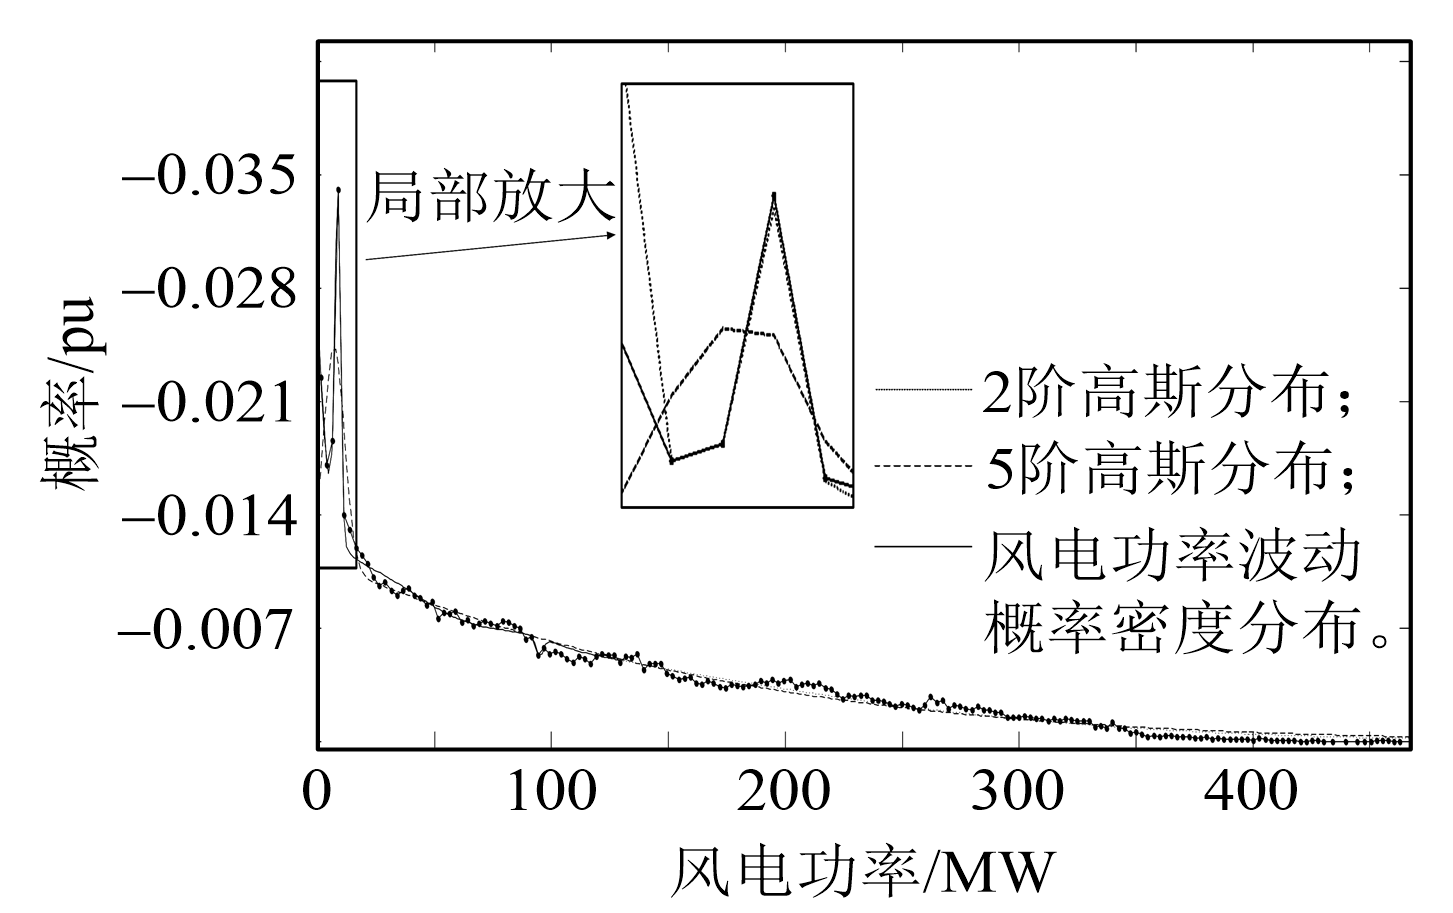
\includegraphics[width = 0.3\textwidth]{figures/功率波动概率密度分布拟合曲线}}
    \hfill
    \subcaptionbox{subcaption3}{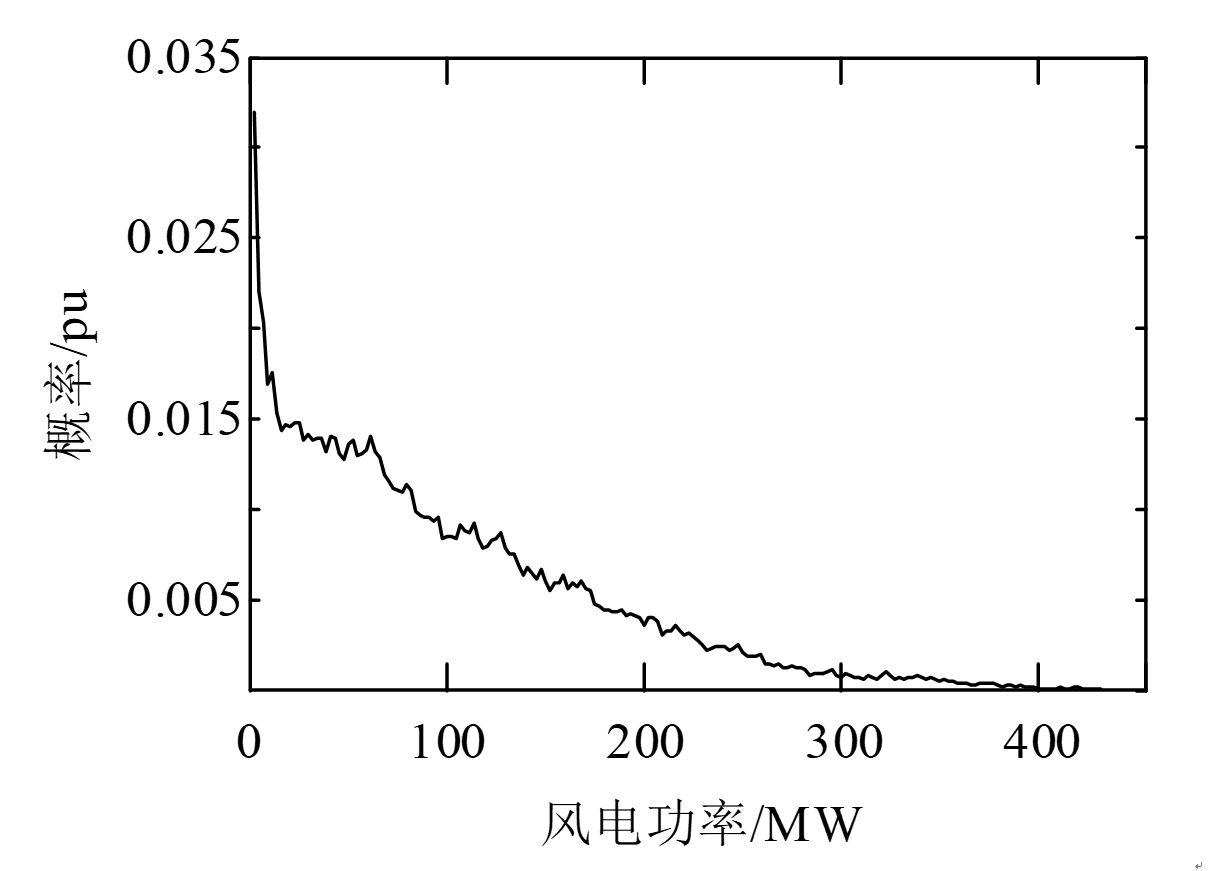
\includegraphics[width = 0.3\textwidth]{figures/功率波动概率密度分布曲线}} 
  \caption{caption}
  \label{fig:label}
  \end{figure*}



正文中的表。(采用三线表,表题为五号宋体,表中为小五宋体。表题在表上方,居中)



\begin{table}[!ht]
    \centering
    \caption{一个只有引脚注释的表}
    \label{tab1}
    \vspace{-0.8em}
\begin{tabular}{ccccccccc}
    %\begin{longtable}{ccccccccc}
        % 表格“首页”显示内容
        %\toprule
        %流型 & IMF1 & IMF2 & IMF 3 & IMF4 & IMF5 & IMF6 & IMF7 & IMF8 \\
        %\midrule
        %\endfirsthead
        % “后续页面”表头显示内容
        %\caption*{\raggedleft 续表~\thetable\quad
        %\hspace{9.5em}          %调整“续表XX”位置在表格右上方
        %} \\
        %\toprule
        %流型 & IMF1 & IMF2 & IMF 3 & IMF4 & IMF5 & IMF6 & IMF7 & IMF8 \\
        %\midrule
        %\endhead
        % 表格“尾页前”,表格最后显示内容
        %\bottomrule
        %\endfoot
        % 表格“尾页”,表格最后显示内容
        %\bottomrule
        %\endlastfoot
    \toprule
      %流型 & IMF1 & IMF2 & IMF 3 & IMF4 & IMF5 & IMF6 & IMF7 & IMF8 \\

      \makebox[0.0823\textwidth][c]{流型} & \makebox[0.0823\textwidth][c]{IMF1} & \makebox[0.0823\textwidth][c]{IMF2} & \makebox[0.0823\textwidth][c]{IMF3} & \makebox[0.0823\textwidth][c]{IMF4} & \makebox[0.0823\textwidth][c]{IMF5} & \makebox[0.0823\textwidth][c]{IMF6} & \makebox[0.0823\textwidth][c]{IMF7} & \makebox[0.0823\textwidth][c]{IMF8} \\
    \midrule
      A & .5284 & .3418 & .0550 & .0449 & .0175 & .0026 & .0039 & .0058 \\
      A & .5326 & .3416 & .0571 & .0423 & .0155 & .0024 & .0036 & .0059 \\
      B & .4580 & .3080 & .0914 & .0623 & .0312 & .0323 & .0096 & .0082 \\
      B & .4542 & .3160 & .0919 & .0646 & .0345 & .0226 & .0068 & .0095 \\
      C & .5782 & .2105 & .1041 & .0439 & .0476 & .0053 & .0077 & .0028 \\
      C & .5762 & .2155 & .1006 & .0421 & .0502 & .0043 & .0087 & .0034 \\
    \bottomrule
%    \end{longtable}
\end{tabular}\\
    \raggedright
    {\footnotesize
    %\hspace{1em}           %调整注释位置
    注1:This footnote shows what footnote symbols to use.
    }
\end{table}






%表使用的注在三线表左下方顶格编写,同用小五宋体
%表,过后添加

\clearpage

%\ifx\allfiles\undefined
%如果有这一部分的参考文献可以放这里
%没有的话不需要
%因此各个部分的参考文献可以分开
%也可以统一放在主文件末尾

%bibfile.bib是放置参考文献的文件,可以用Zotero导出
%bibliography{bibfile}
%\end{document}

%\else
%\fi
